\subsection{Схема разработанного вентиля}
\subsubsection{Описание}
Разработанный NOR-вентиль реализован на КМОП-транзисторах и состоит из пары p-канальных (\( M_1 \), \( M_2 \)) и n-канальных (\( M_3 \), \( M_4 \)) транзисторов. Вентиль выдаёт логическую $"1"$ на выходе \( \text{Out} \), только когда оба входа \( A \) и \( B \) находятся в $"0"$. При подаче $"1"$ на любой из входов nMOS транзисторы подключают выход к земле (GND), устанавливая $"0"$ на выходе, выполняя функцию NOR.

\subsubsection{Схема NOR-вентиля}
\begin{figure}[H]
	\centering
	\begin{circuitikz}[european, scale=1.5, transform shape]
		\draw (0,0)
		-- (4,0) to[short, *-] (4,0)
		-- (10,0) node[right] {$\small V_{\text{\scriptsize DD}}$};

		\draw (0,-5.5)
		-- (4,-5.5) to[short, *-] (4,-5.5)
		-- (10,-5.5) node[right] {\small GND};

		\draw (4,0) -- (4, -0.23)
		++(0, -0.77) node[pmos,emptycircle]{\small $M_1$} (4, -1.5)
		++ (0, -1.05) node[pmos,emptycircle]{\small $M_2$} (4,-3)
		++(0, -0.325) --(4, -3.41)
		++(0, -1.055) node[nmos,emptycircle]{\small $M_3$} (4, -5)
		++(0, -0.24) -- (4, -5.5);

		\draw
		(1, -1) node[left]{\small $A$}
		-- (3.015, -1);

		\draw (2.5, -1)
		to [short, *-] (2.5, -1)
		-- (2.5, -2.41)
		++ (0, -0.28)
		-- (2.5, -3.55)
		-- (3.861, -3.55) ++(0.139, 0) node[jump crossing] ++(0.14, 0)
		-- (5.3, -3.55)
		-- (5.3, -4.275)
		-- (5.525, -4.275);

		\draw
		(1, -2.55) node[left]{\small $B$}
		-- (2.36, -2.55) ++(0.14, 0) node[jump crossing] (2.55, -2.55)
		++(0.14, 0) -- (3.016, -2.55);

		\draw (2, -2.55)
		to [short, *-] (2, -2.55)
		-- (2, -4.465) -- (3.02, -4.465);

		\draw (6.5, -5.5)
		to [short, *-] (6.5, -5.5)
		-- (6.5, -5.05)
		++(0, 0.775) node[nmos,emptycircle]{\small $M_4$} (6.5, -3.5)
		-- (6.5, -2.75)
		to[short, *-] (6.5, -2.75);

		\draw (5, -2.75)
		-- (10, -2.75) node[right] {\small Out};

		\draw (4, -3.2)
		to[short, *-] (4, -3.2)
		-- (5, -3.2)
		-- (5, -2.75);

	\end{circuitikz}
	\caption{NOR вентиль на nMOS и pMOS транзисторах}
\end{figure}


\subsection{Символ вентиля}
\begin{figure}[H]
	\centering
	\begin{circuitikz}[european, scale=2.5, transform shape]
		\draw[thick] node[ieeestd nor port] (N) {};
		\draw[thick] (N.up) -- ++(0, 0.3) ++(0, 0.2) node[up] {\scriptsize $V_{\text{DD}}$}
		\draw[thick] (N.left) ++ (-0.3, 0.3) node[left] {\scriptsize $A$}
		\draw[thick] (N.left) ++ (-0.3, -0.3) node[left] {\scriptsize $B$}
		\draw[thick] (N.N-not) ++ (1, 0) node[right] {\scriptsize Out}
	\end{circuitikz}
	\caption{символ NOR вентиля на nMOS и pMOS транзисторах}
\end{figure}


\subsection{Схема тестирования}
\begin{figure}[H]
	\centering
	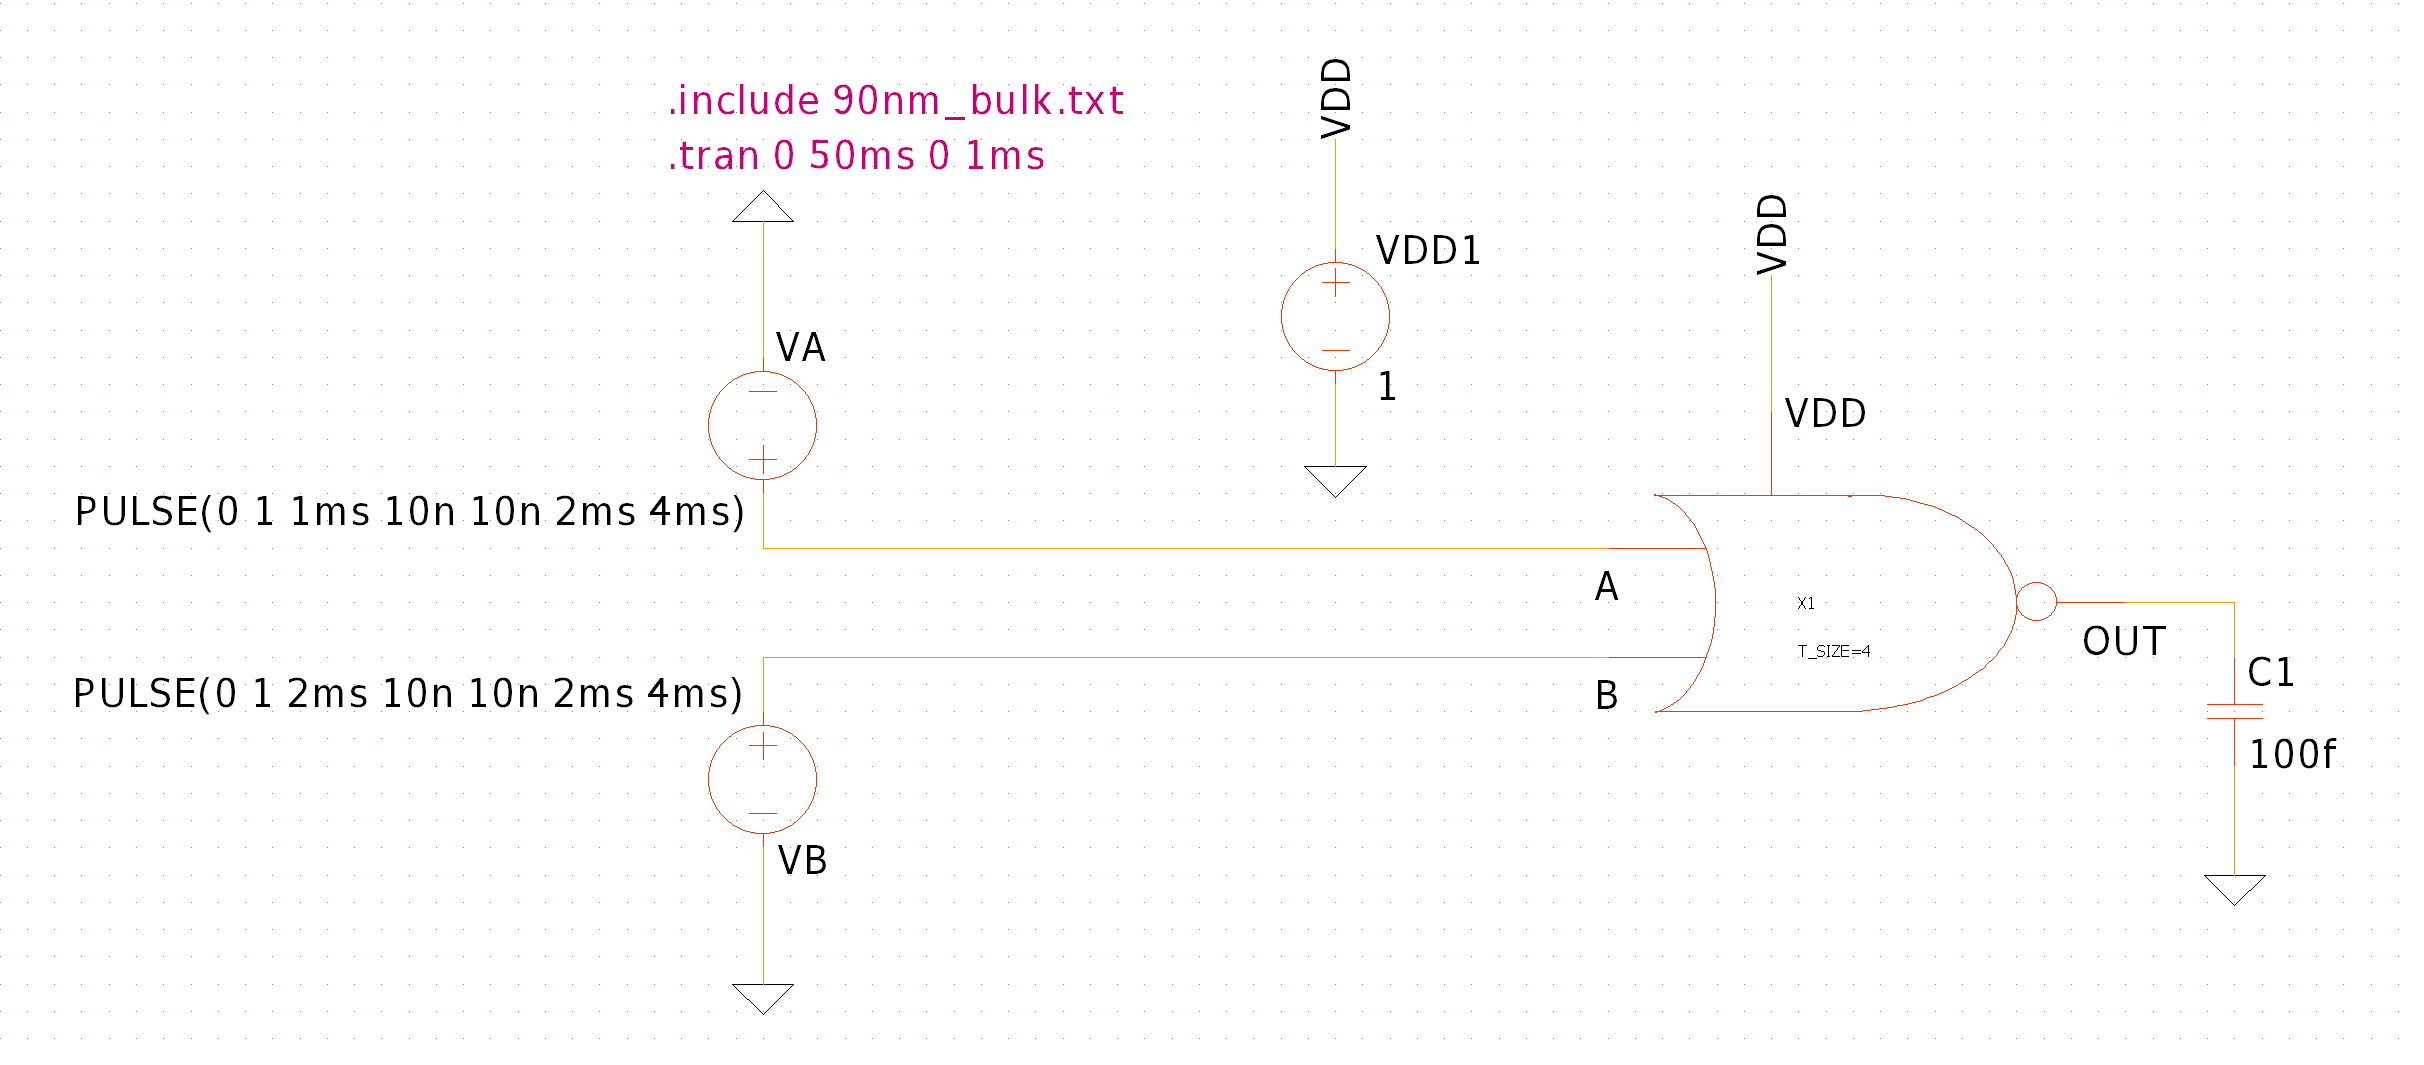
\includegraphics[width=1\textwidth]{../data/test_cmos_nor}
	\caption{Схема тестирования разработанного NOR-вентиля}
\end{figure}


\subsection{Временная диаграмма тестирования вентиля}
\setlength{\columnsep}{1cm}

\begin{multicols}{2}
	Тестируемый NOR-элемент должен соответствовать следующей таблице истинности.

	Временная диаграмма на Рисунке 4 показывает изменение напряжений на входах \( A \), \( B \) и выходе \( \text{Out} \) во времени, подтверждая правильность работы NOR-элемента.

	\columnbreak

	\noindent
	\renewcommand{\arraystretch}{1.33}
	\raggedright
	\begin{tabular}{|>{\centering\arraybackslash}p{1.2cm}|>{\centering\arraybackslash}p{1.2cm}|>{\centering\arraybackslash}p{1.6cm}|}
		\hline
		A & B & Out \\
		\hline
		0 & 0 & 1   \\
		0 & 1 & 0   \\
		1 & 0 & 0   \\
		1 & 1 & 0   \\
		\hline
	\end{tabular}

\end{multicols}

\begin{figure}[H]
	\centering
	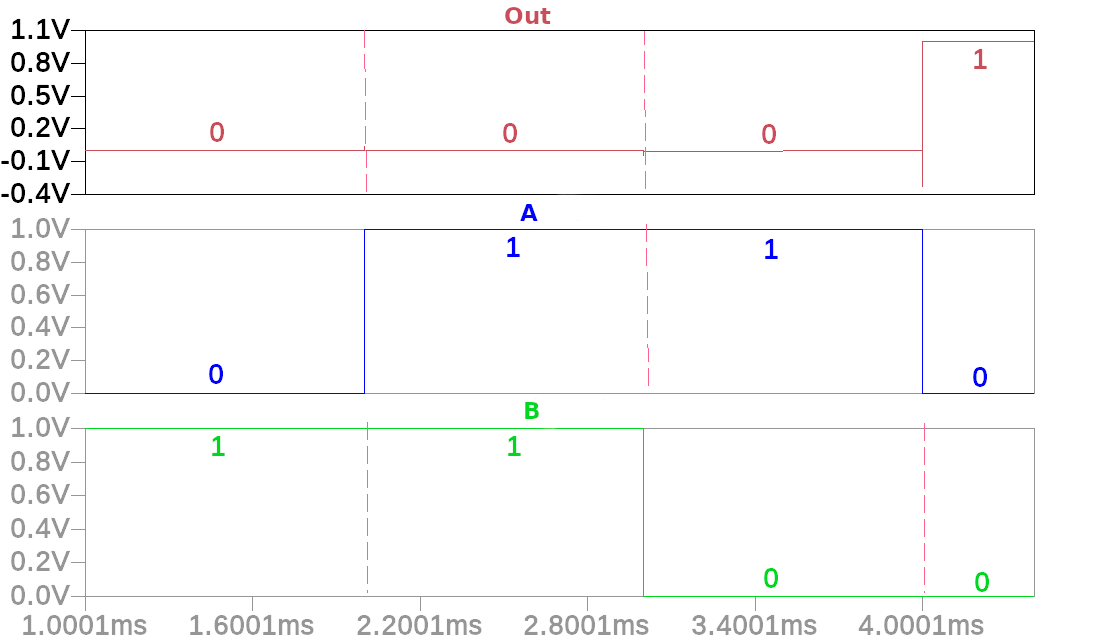
\includegraphics[width=0.8\textwidth]{../data/test_cmos_nor_time}
	\caption{Временная диаграмма напряжений на A, B, Out}
\end{figure}


\subsection{Результат измерения задержки распространения сигнала через вентиль}
\subsubsection{Теоретическая основа}
Задержка распространения сигнала была измерена на временной диаграмме (см. Рис. 5 и Рис. 6 с увеличенным масштабом). Величина задержки измеряется от момента, когда входной сигнал достигает уровня в 50\% от установившегося до момента достижения уровня 50\% выходным сигналом. Уровень 50\% - это точка, в которой сигнал находится ровно посередине между низким и высоким логическими уровнями, поэтому такой уровень служит теоретической $"\text{отсечкой}"$ задержки. Таким образом, задержка схемы это среднее задержек переднего и заднего фронтов сигнала

\subsubsection{Временные диаграммы задержек переднего и заднего фронтов}
\setlength{\columnsep}{2.5cm}

\begin{multicols}{2}

	\begin{figure}[H]
		\centering
		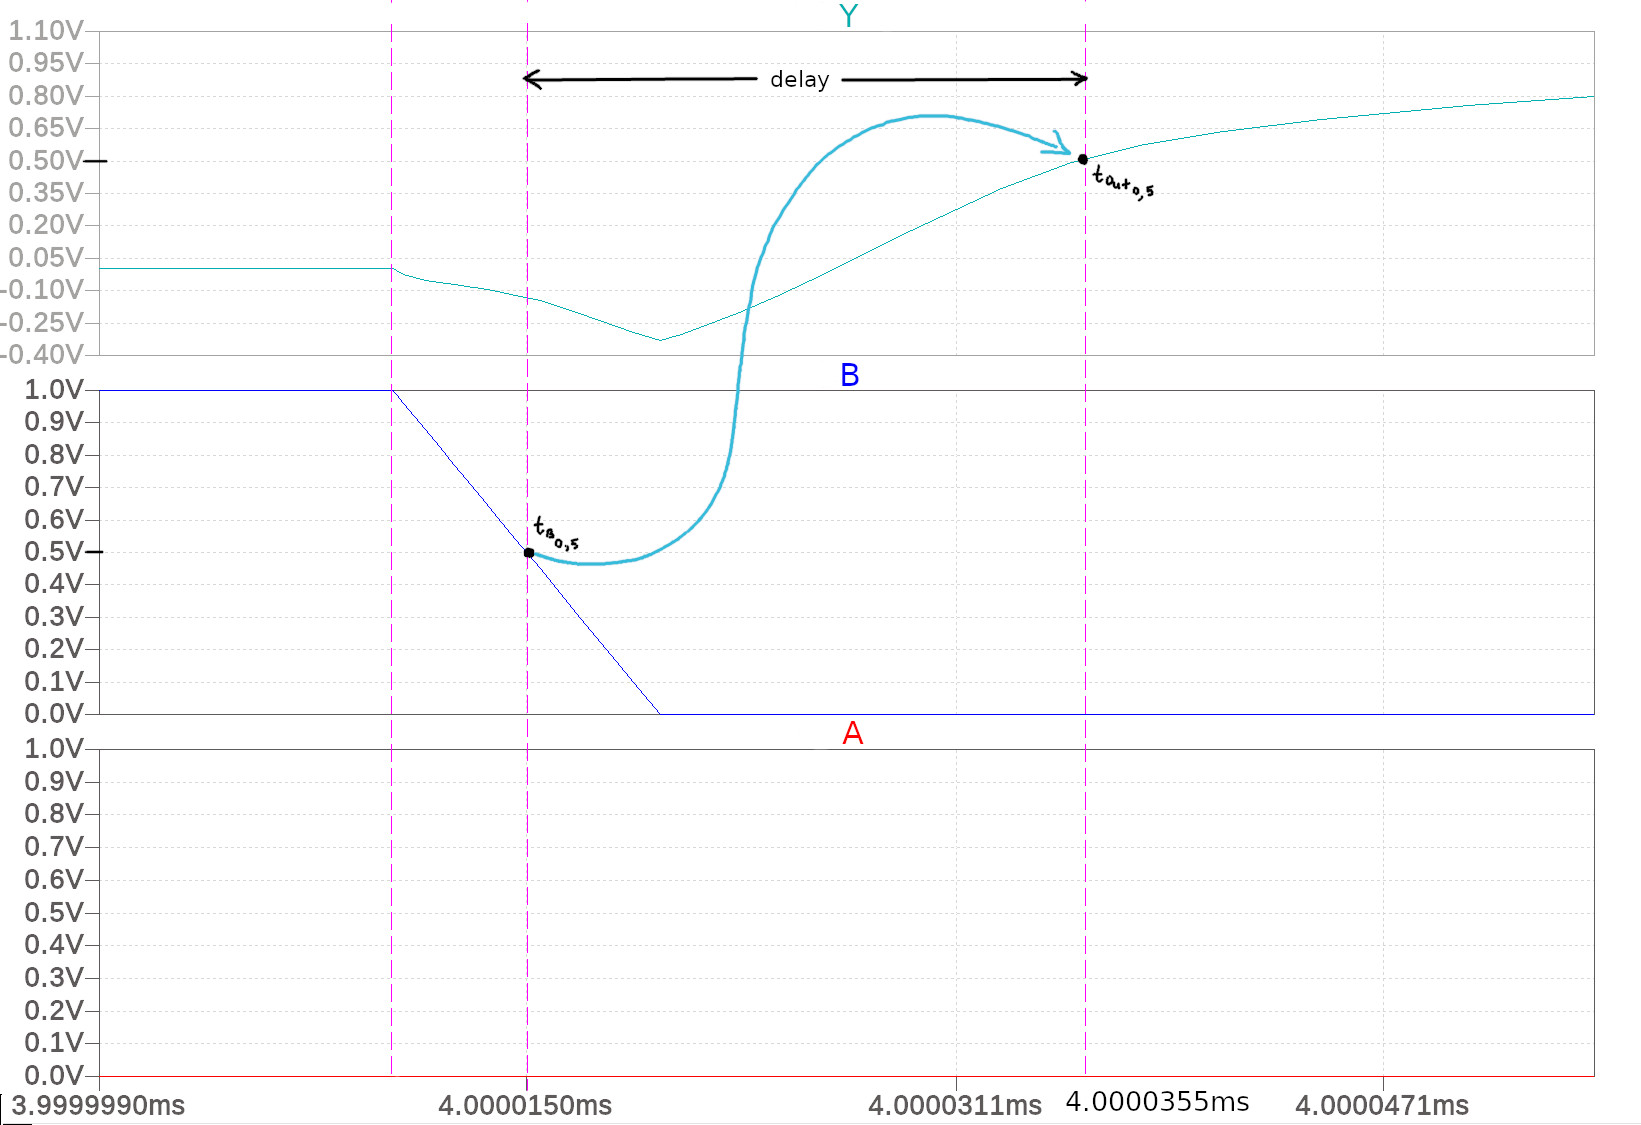
\includegraphics[width=0.58\textwidth]{../data/nor_front_delay.png}
		\captionsetup{width=1\textwidth}
		\centering
		\caption{Передний~фронт~сигнала~Y}
	\end{figure}

	\begin{figure}[H]
		\centering
		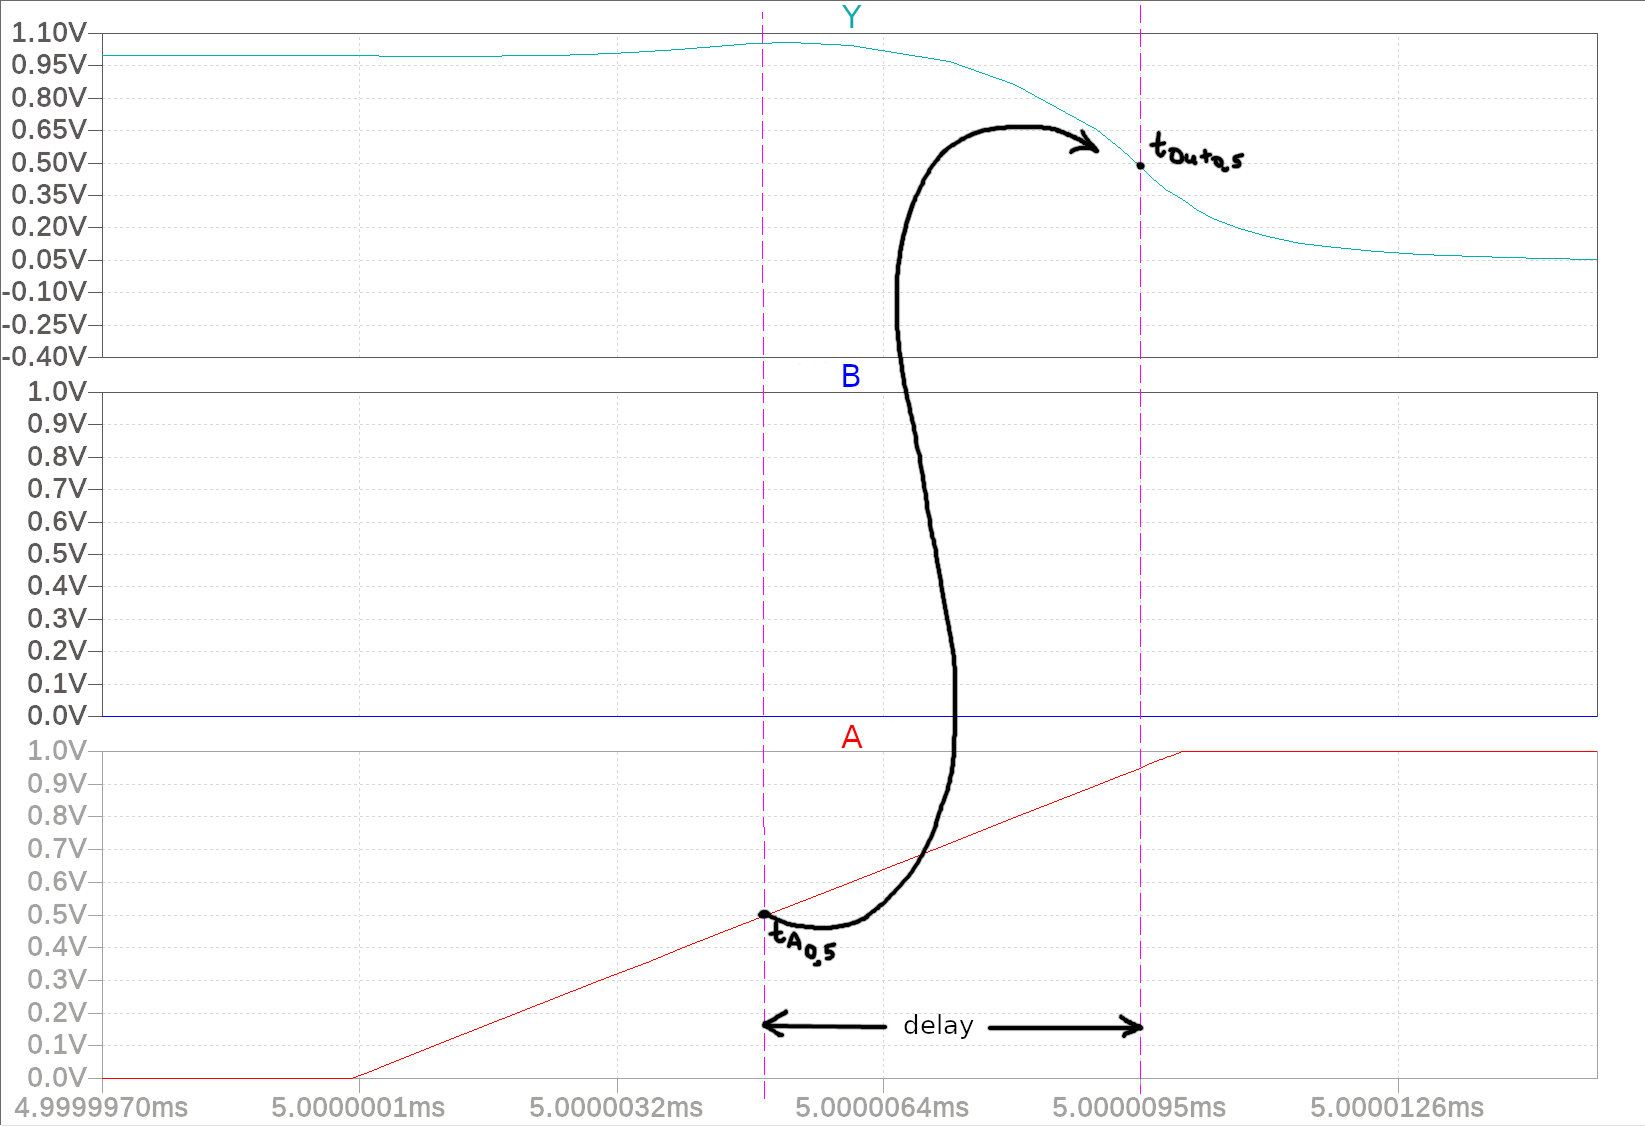
\includegraphics[width=0.6\textwidth]{../data/nor_back_delay.png}
		\caption{Задний фронт сигнала Y}
	\end{figure}

	\columnbreak

	\centering
	\vspace*{0.9cm}
	Расчёт задержек:

	\vspace*{-0.3cm}
	\[
		\begin{gathered}
			t_{Y_{0.5}} = 4.0000355 \, \text{мс} \\
			t_{B_{0.5}} = 4.000015 \, \text{мс} \\
			t_{pd_\uparrow} = 20.5 \, \text{нс} \\
		\end{gathered}
	\]

	\vspace*{5cm}
	Расчёт задержек:

	\vspace*{-0.3cm}
	\[
		\begin{gathered}
			t_{Y_{0.5}} = 5.0000095 \, \text{мс} \\
			t_{A_{0.5}} = 5.000005 \, \text{мс} \\
			t_{pd_\downarrow} = 4.5 \, \text{нс} \\
		\end{gathered}
	\]
\end{multicols}

\subsubsection{Расчёт задержки распространения схемы}
Исходя из задержек переднего и заднего фронтов:

\[
	t_{pd} = \frac{t_\uparrow + t_\downarrow}{2} = \frac{20.5+4.5}{2} = 12.5 \, \text{нс}
\]


\subsection{Максимальная частота работы вентиля}
Максимальная частота работы вентиля рассчитывается по формуле:

\[
	f_{max} = \frac{1}{t_{pd}}
\]

Подставив \( t_{pd} = 12.5 \, \text{нс} \), получаем:

\[
	f_{max} = \frac{1}{12.5 \cdot 10^{-9}} = 80 \, \text{МГц}
\]

Следовательно, максимальная частота работы вентиля составляет \( 80 \, \text{МГц} \).


\subsection{Схема разработанного БОЭ}
% \begin{figure}[H]
% 	\centering
% 	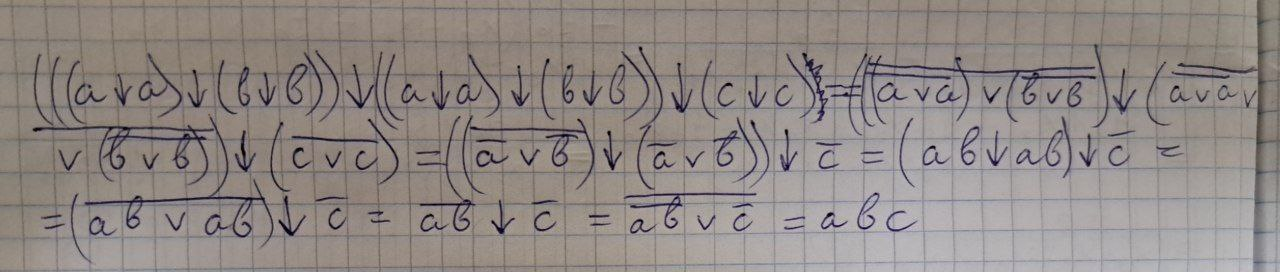
\includegraphics[width=1\textwidth]{../data/formula}
% 	\caption{Вывод схемы БОЭ}
% \end{figure}

\subsubsection{Вывод схемы БОЭ}

Для каждого выхода \( Z_i \) на основе таблицы истинности строим логическое выражение в базисе ИЛИ-НЕ.

### Выражение для \( Z_0 \):
\[
	\begin{gathered}
		Z_0 = \overline{S_1} \cdot \overline{S_0} \cdot Y = \overline{(S_0 \vee S_1) \vee \overline{Y}} = (\overline{\overline{S_0 \vee S_1}}) \vee \overline{Y} \\
		Z_0 = ((S_0 \downarrow S_1) \downarrow (S_0 \downarrow S_1)) \downarrow (Y \downarrow Y)
	\end{gathered}
\]

### Выражение для \( Z_1 \):
\[
	\begin{gathered}
		Z_1 = \overline{S_1} \cdot S_0 \cdot Y = \overline{(S_1 \vee \overline{S_0}) \vee \overline{Y}} = (\overline{S_1 \vee \overline{S_0}}) \vee \overline{Y} \\
		Z_1 = ((S_1 \downarrow (S_0 \downarrow S_0)) \downarrow (S_1 \downarrow (S_0 \downarrow S_0))) \downarrow (Y \downarrow Y)
	\end{gathered}
\]

### Выражение для \( Z_2 \):
\[
	\begin{gathered}
		Z_2 = S_1 \cdot \overline{S_0} \cdot Y = \overline{(\overline{S_1} \vee S_0) \vee \overline{Y}} = (\overline{\overline{S_1} \vee S_0}) \vee \overline{Y} \\
		Z_2 = (((S_1 \downarrow S_1) \downarrow S_0) \downarrow ((S_1 \downarrow S_1) \downarrow S_0)) \downarrow (Y \downarrow Y)
	\end{gathered}
\]

### Выражение для \( Z_3 \):
\[
	\begin{gathered}
		Z_3 = S_1 \cdot S_0 \cdot Y = \overline{(\overline{S_1} \vee \overline{S_0}) \vee \overline{Y}} = (\overline{\overline{S_1} \vee \overline{S_0}}) \vee \overline{Y} \\
		Z_3 = (((S_1 \downarrow S_1) \downarrow (S_0 \downarrow S_0)) \downarrow ((S_1 \downarrow S_1) \downarrow (S_0 \downarrow S_0))) \downarrow (Y \downarrow Y)
	\end{gathered}
\]

Таким образом, конечные формулы для каждого \( Z_i \) выражены в базисе ИЛИ-НЕ, что соответствует структуре демультиплексора 1 в 4 на базе логического элемента NOR.

Реализация этих логических выражений с использованием NOR-вентиля выглядит следующим образом:

1. Для инверсии сигналов \( S_1 \) и \( S_0 \) используются NOR-вентиля с одинаковыми входами:
\[
	\overline{S_0} = NOR(S_0, S_0), \quad \overline{S_1} = NOR(S_1, S_1)
\]

2. Логические операции для каждого выхода можно развернуть через NOR следующим образом:

\[
	Z_0 = NOR(NOR(NOR(S_1, S_0), NOR(S_1, S_0)), NOR(Y, Y))
\]
\[
	Z_1 = NOR(NOR(NOR(S_1, \overline{S_0}), NOR(S_1, \overline{S_0})) , NOR(Y, Y))
\]
\[
	Z_2 = NOR(NOR(NOR(\overline{S_1}, S_0), NOR(\overline{S_1}, S_0)) , NOR(Y, Y))
\]
\[
	Z_3 = NOR(NOR(NOR(\overline{S_1}, \overline{S_0}), NOR(\overline{S_1}, \overline{S_0})) , NOR(Y, Y))
\]

Таким образом, каждый выход \( Z_i \) активен при соответствующей комбинации управляющих сигналов \( S_1, S_0 \), что реализует функцию демультиплексора на базе NOR-вентиля.

\subsubsection{Схема БОЭ}

\begin{figure}[H]
	\centering
	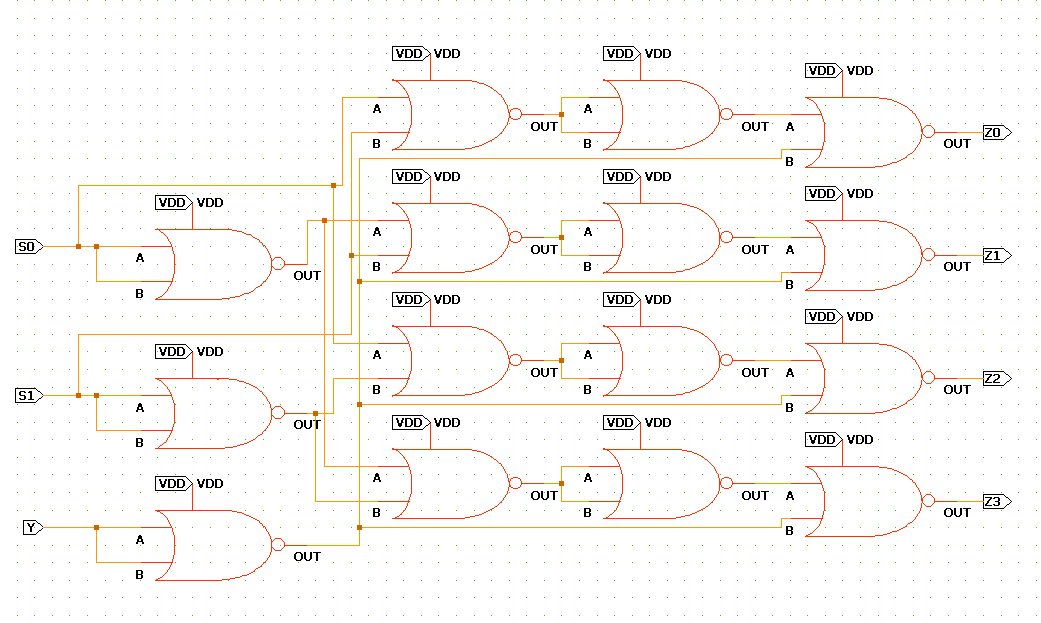
\includegraphics[width=1\textwidth]{../data/demultiplexer_1_to_4}
	\caption{Демультиплексор «1 в 4»}
\end{figure}


\subsection{Символ разработанного БОЭ}
\begin{figure}[H]
	\centering
	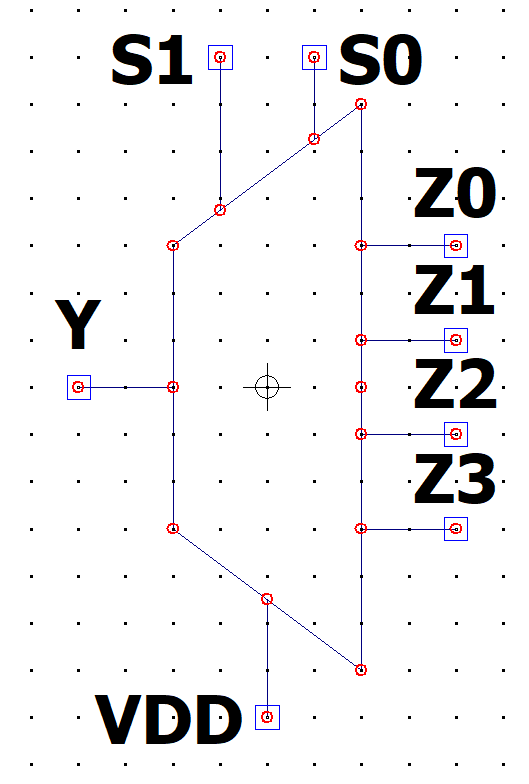
\includegraphics[width=0.4\textwidth]{../data/demux}
	\caption{Символ Демультиплексора <<1 в 4>>}
\end{figure}


\subsection{Схема тестирования разработанного БОЭ}
\begin{figure}[H]
	\centering
	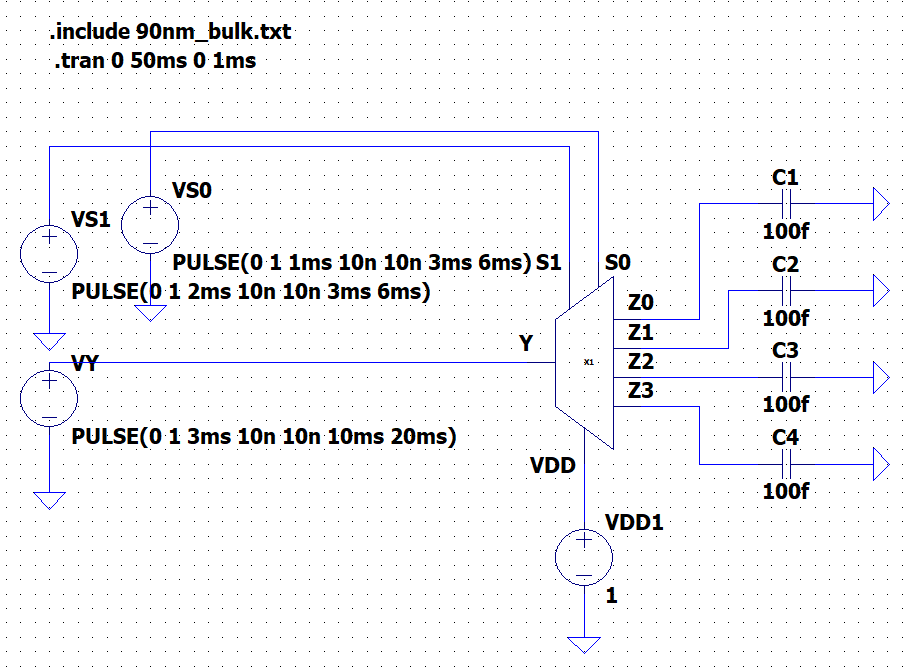
\includegraphics[width=1\textwidth]{../data/boe-testing}
	\caption{Схема тестирования Демультиплексора <<1 в 4>>}
\end{figure}


\subsection{Временная диаграмма тестирования БОЭ}
\setlength{\columnsep}{1cm}

\begin{multicols}{2}
	Тестируемый демультиплексор 1-в-4 должен соответствовать следующей таблице истинности, где \( Y \) — вход, \( S_1 \) и \( S_2 \) — управляющие сигналы, а \( Z_0 \), \( Z_1 \), \( Z_2 \) и \( Z_3 \) — выходы.

	Временная диаграмма на Рисунке 10 показывает изменение напряжений на входах \( Y \), \( S_1 \), \( S_2 \) и выходах \( Z_0 \), \( Z_1 \), \( Z_2 \), \( Z_3 \) во времени, подтверждая правильность работы демультиплексора.

	\columnbreak

	\noindent
	% \vspace*{0.1cm}
	\renewcommand{\arraystretch}{1.12}
	\raggedright
	\begin{tabular}{|>{\centering\arraybackslash}p{0.8cm}|>{\centering\arraybackslash}p{0.8cm}|>{\centering\arraybackslash}p{0.8cm}|>{\centering\arraybackslash}p{0.8cm}|>{\centering\arraybackslash}p{0.8cm}|>{\centering\arraybackslash}p{0.8cm}|>{\centering\arraybackslash}p{0.8cm}|}
		\hline
		$S_1$ & $S_2$ & $Y$ & $Z_0$ & $Z_1$ & $Z_2$ & $Z_3$ \\
		\hline
		0     & 0     & 1   & 1     & 0     & 0     & 0     \\
		0     & 1     & 1   & 0     & 1     & 0     & 0     \\
		1     & 0     & 1   & 0     & 0     & 1     & 0     \\
		1     & 1     & 1   & 0     & 0     & 0     & 1     \\
		\hline
		0     & 0     & 0   & 0     & 0     & 0     & 0     \\
		0     & 1     & 0   & 0     & 0     & 0     & 0     \\
		1     & 0     & 0   & 0     & 0     & 0     & 0     \\
		1     & 1     & 0   & 0     & 0     & 0     & 0     \\
		\hline
	\end{tabular}

\end{multicols}

\begin{figure}[H]
	\centering
	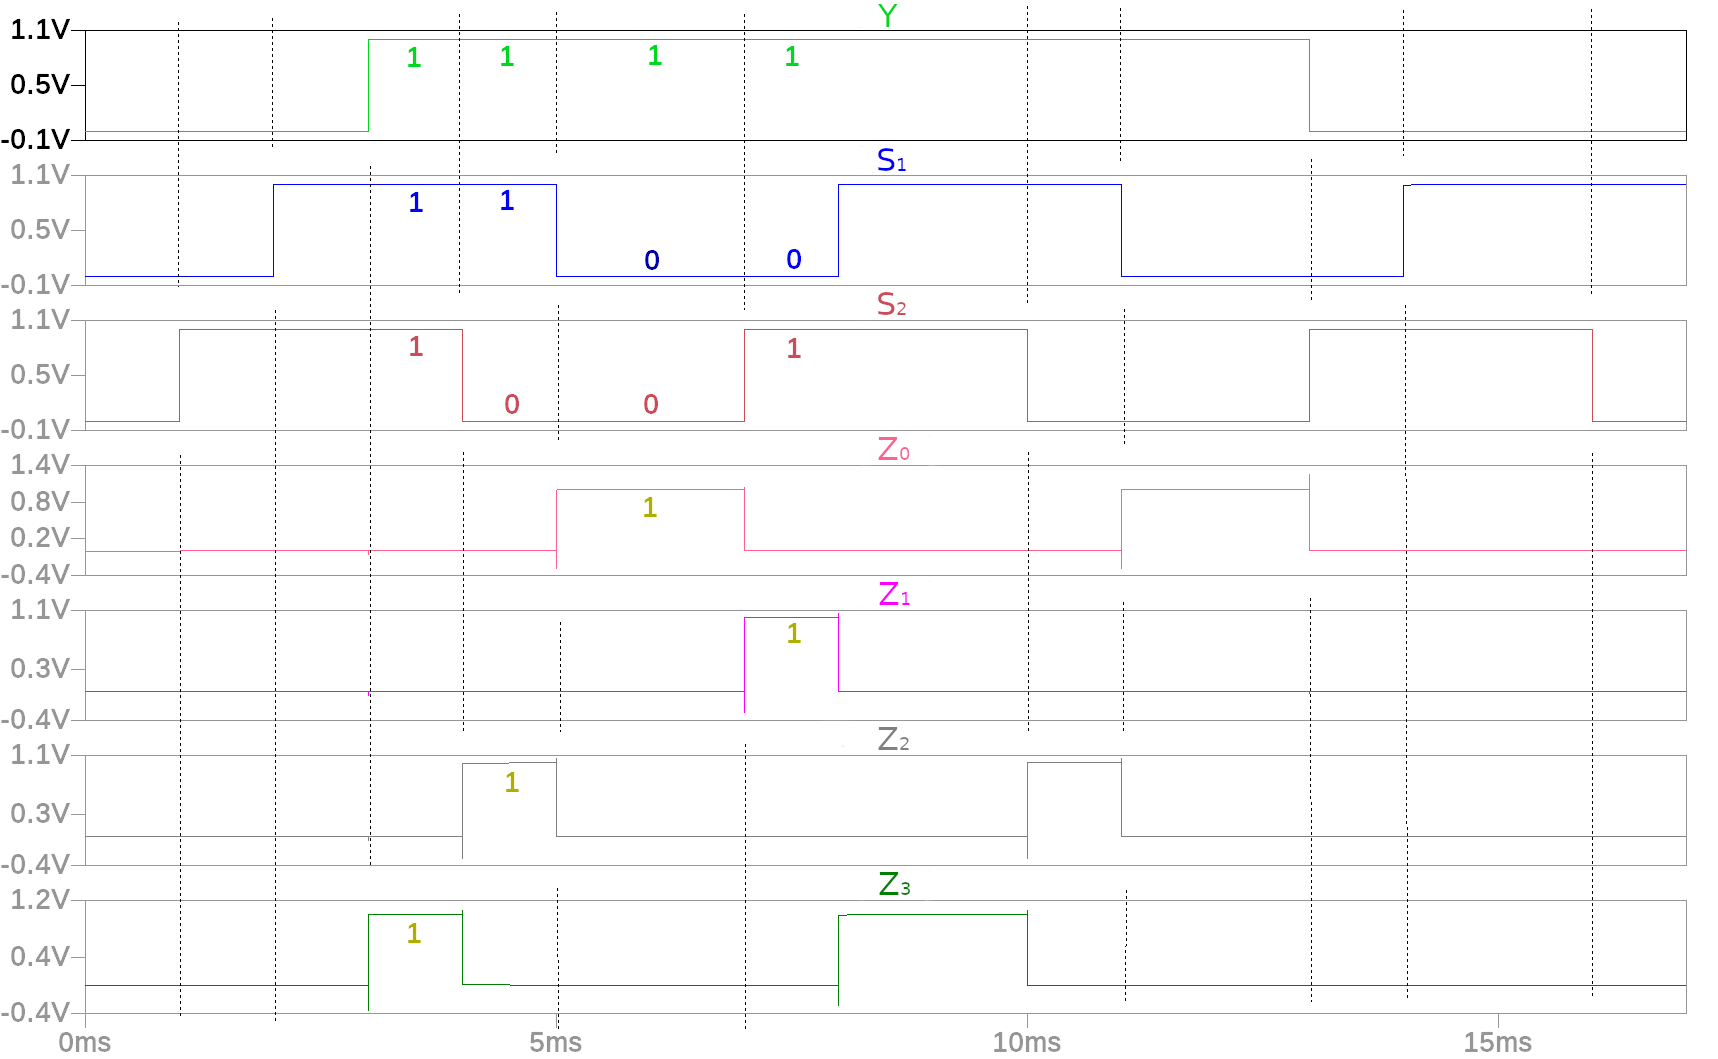
\includegraphics[width=1\textwidth]{../data/test_boe_time}
	\caption{Временная диаграмма напряжений на $Z_0, Z_1, Z_2, Z_3, S_1, S_2, Y$}
\end{figure}


\subsection{Результат измерения задержки распространения сигнала через БОЭ}
\subsubsection{Теоретическая основа}
Задержка распространения сигнала в БОЭ Демультиплексор <<1 в 4>> была измерена аналогично измерению задержки NOR-вентиля, при этом стоит отметить, что минимальное теоретическое значение задержки распространения в БОЭ Демультиплексор <<1 в 4>> можно вычислить основываясь на эмпирически найденном ранее значении задержки NOR-вентиля, не прибегая к измерению на временной диаграмме. Критический путь - это самый длинный путь, с наибольшей задержкой, от входа к выходу. В комбинационных схемах задержка распространения определяется \textit{суммой задержек распространения элементов в \textbf{критическом пути}}. В нашей реализации Демультиплексора <<1 в 4>> критический путь составляет 4 NOR-вентиля, следовательно, минимальная теоретическая задержка распространения должна получиться \textbd{в 4 раза больше}: \(t_{pd} = 4 \cdot t_{pd_{NOR}} = 4 \cdot 12.5 = 50 \, \text{нс}.\)

\subsubsection{Временные диаграммы задержек переднего и заднего фронтов}
\setlength{\columnsep}{2.6cm}

\begin{multicols}{2}

	\begin{figure}[H]
		\centering
		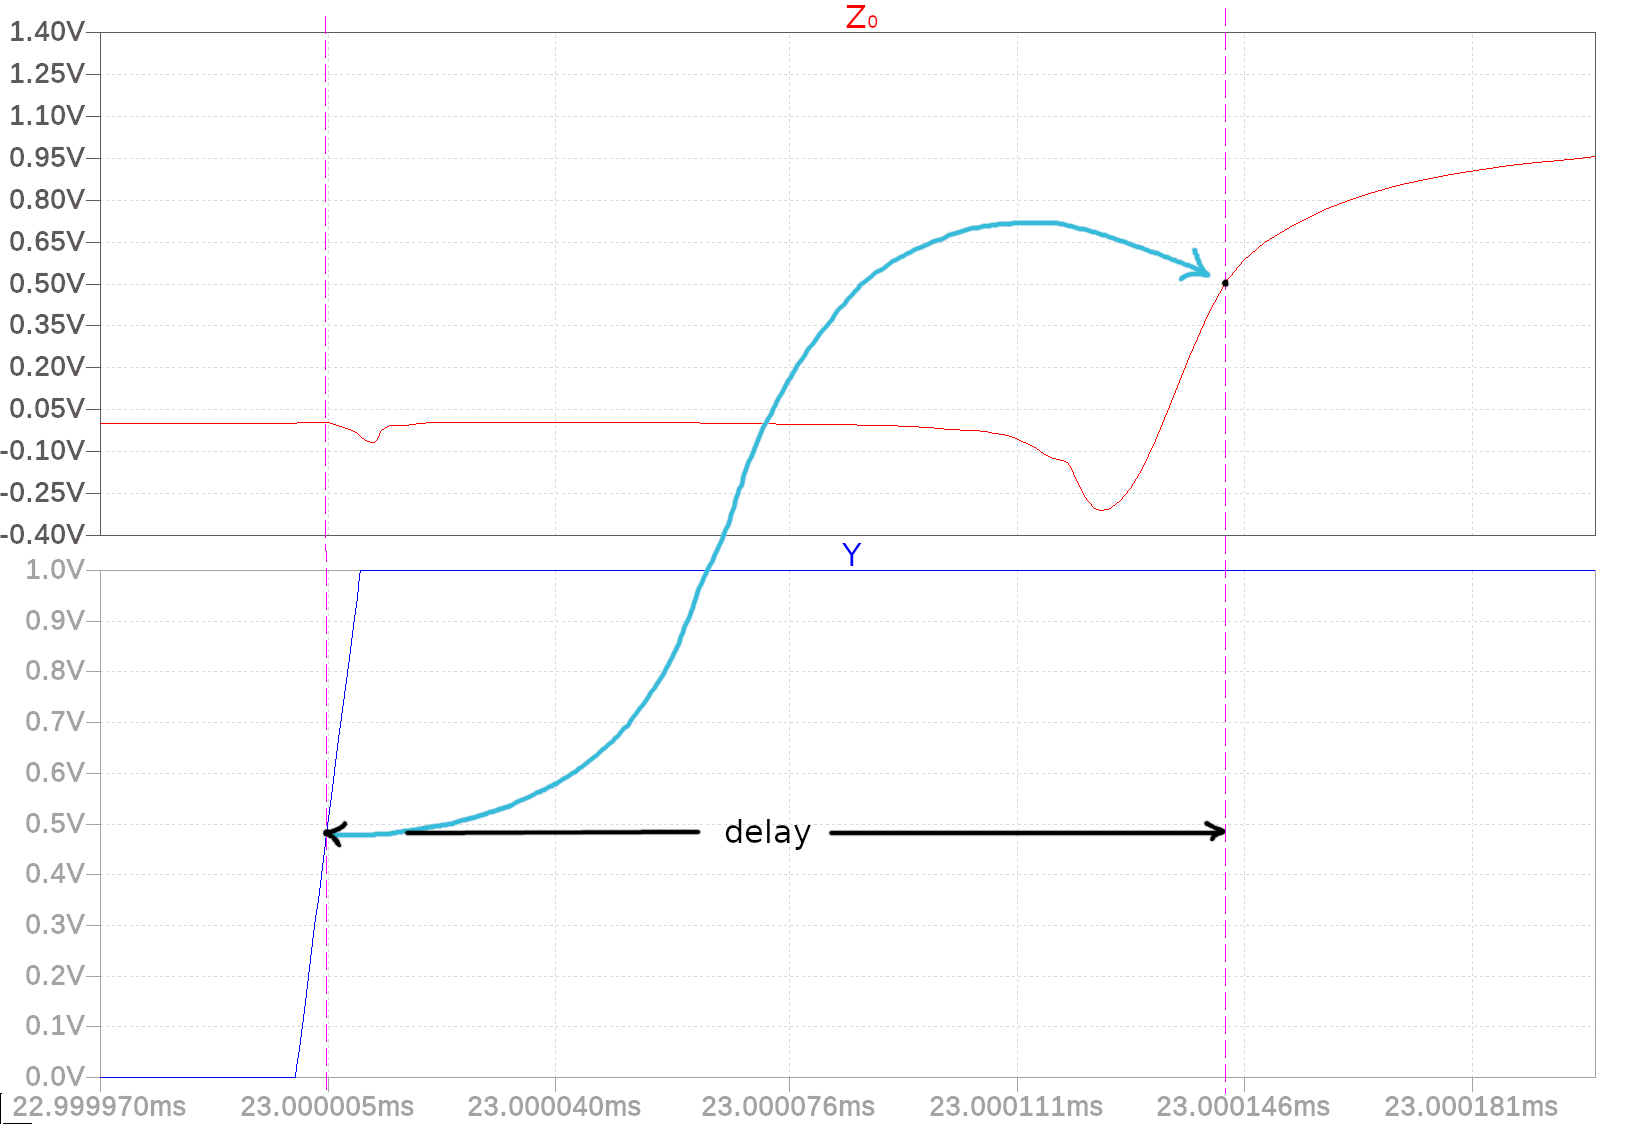
\includegraphics[width=0.6\textwidth]{../data/boe_front_delay.png}
		\captionsetup{width=1\textwidth}
		\centering
		\caption{Передний фронт сигнала Z_0}
	\end{figure}

	\begin{figure}[H]
		\centering
		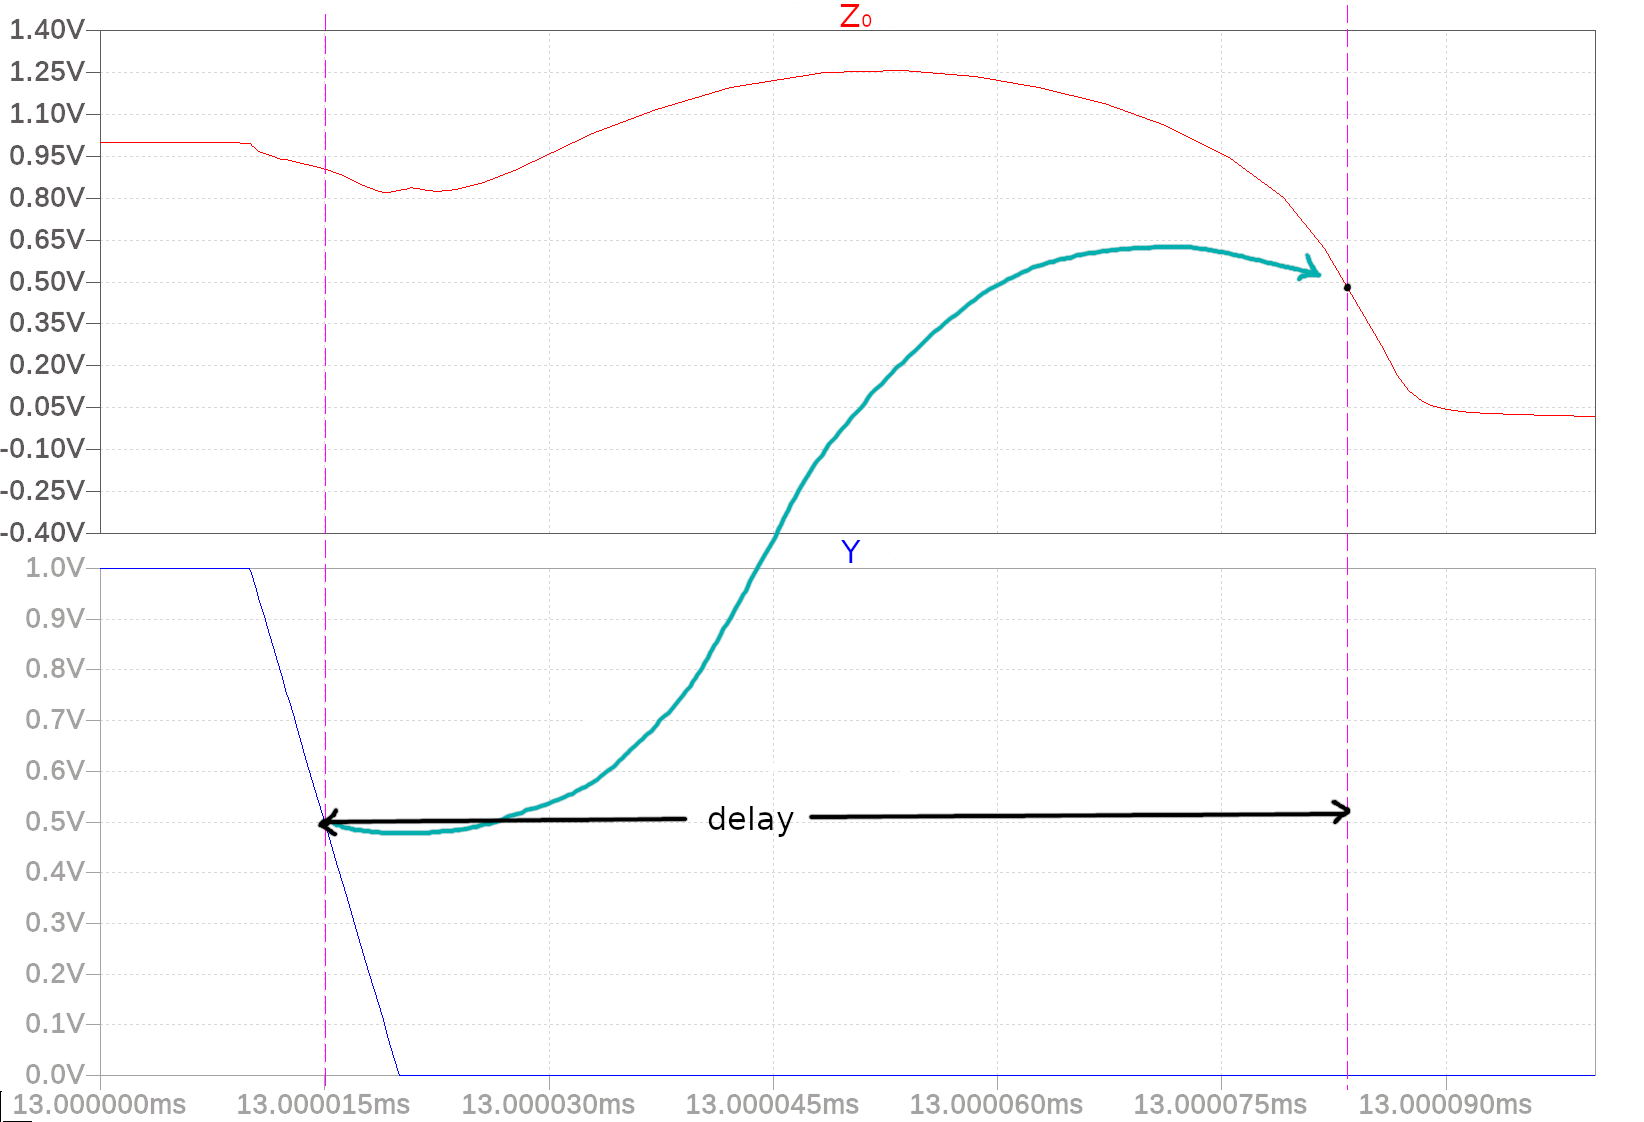
\includegraphics[width=0.6\textwidth]{../data/boe_back_delay.png}
		\captionsetup{width=1\textwidth}
		\centering
		\caption{Задний фронт сигнала Z_0}
	\end{figure}

	\columnbreak

	\centering
	\vspace*{0.9cm}
	Расчёт задержек:

	\vspace*{-0.3cm}
	\[
		\begin{gathered}
			t_{Y_{0.5}} = 13.000015 \, \text{мс} \\
			t_{B_{0.5}} = 13.000083 \, \text{мс} \\
			t_{pd_\uparrow} = 68 \, \text{нс} \\
		\end{gathered}
	\]

	\vspace*{5cm}
	Расчёт задержек:

	\vspace*{-0.3cm}
	\[
		\begin{gathered}
			t_{Y_{0.5}} = 23.000005 \, \text{мс} \\
			t_{A_{0.5}} = 23.000143 \, \text{мс} \\
			t_{pd_\downarrow} = 138 \, \text{нс} \\
		\end{gathered}
	\]
\end{multicols}

\subsubsection{Расчёт задержки распространения схемы}
Исходя из задержек переднего и заднего фронтов:

\[
	t_{pd} = \frac{t_\uparrow + t_\downarrow}{2} = \frac{68+138}{2} = 103 \, \text{нс}
\]


\subsection{Максимальная частота работы БОЭ}
Максимальная частота работы Демультиплексора <<1 в 4>> рассчитывается по формуле:

\[
	f_{max} = \frac{1}{t_{pd}}
\]

Подставив \( t_{pd} = 103 \, \text{нс} \), получаем:

\[
	f_{max} = \frac{1}{103 \cdot 10^{-9}} = 9.709 \, \text{МГц}
\]

Следовательно, максимальная частота работы Демультиплексора <<1 в 4>> составляет \( 9.709 \, \text{МГц} \).

